\section{Оценки выхода сигнальных процессов}



В последние десятилетия, среди методов оценки физических эффектов вызванных
прохождением ионизирующего излучения через вещество, получил широкое применение
метод прямого численного моделирования, опирающийся на развитую теорию
методов Монте-Карло.
%TODO: citations

Учёт разнообразных параметров установки (геометрия детекторов, материалы
активных и пассивных частей детекторов) позволяет, в принципе, произвести
моделирование отклика детектирующей системы на фоновые и сигнальные события с
достаточно высокой степенью правдоподобности. Чаще всего экспериментальные
коллаборации располагают набором параметров свойственных определённому
энергетическому диапазону определяющему вполне феноменологию эксперимента,
в рамках которого уточнение и верификация модели производятся итеративно.
Учитываемые физические
процессы и явления при этом по большей части полностью включены в физику
Стандартной модели, и имеют к тому времени заранее определённые области
правдоподобия, определяемые энергией и составом излучения.

В случае исследования новых физических процессов, сложно поддающихся численному
моделированию или вовсе не включённых в Стандартную модель, практический
интерес представляет построение соответствующих генераторов событий (в рамках
методов Монте-Карло): такие программы позволяют произвести моделирование
сигнальных событий как совместно с фоновыми, для оценки параметров установки
(аксептанса, эффективности), так и отдельно, с целью выявления неочевидных
систематических эффектов, сделать достоверные предположения о характере отклика
детекторной системы и получить важные численные оценки для параметров
считывающей аппаратуры и статистики данных.

\subsection{Рождение тёмного фотона в толстой мишени}

Рассмотрим процесс испускания массивной $U(1)'$-частицы $A'$ в конечном или
начальном состоянии электроном рассеивающимся на ядре $Z$. С эффективной точки
зрения, $A'$ удобно рассматривать как эквивалент кванта тормозного излучения
с каплингом к электрону $e \epsilon$ вместо $e$ и массой $m_{A'}$.
Дифференциальное сечение, согласно предполагаемой кинематической картине,
может быть получено в модификации метода Вайтцзаккера-Вильямса выполненной
Кимом и Цаем \cite{KimTsaiWWReview}, через факторизацию на эффективный фотонный
поток, предложенную теми же авторами в 1986 г. в качестве модели для
аналогичного процесса с аксионом в конечном состоянии \cite{tsai.axion}.
В 1924 году Ферми предложил~\cite{Fermi1924}
способ быстрой оценки, который в 1934 году был развит Вайцзеккером и
(независимо) Вильямсом~\cite{Weizsacker1934, Williams1934} показавшим, что для налетающей частицы обладающей массой $M$,
зарядом $Ze$ и энергией $E=\gamma M$ справедливо приближение т.н. эквивалентных
(виртуальных) фотонов со спектральной плотностью $\rho (\omega)$:

\begin{equation}
    \rho ( \omega ) = \frac{Z^2 \alpha}{\pi \omega} ( 2 x K_0 (x) K_1 (x) - x^2 [K_1^2(x) - K_0^2(x) ] ),
    \label{eq:WWSpectrum}
\end{equation}
где $\omega$ соответствует эффективной энергии фотона,
$x = \omega b_{min} / \gamma$ -- минимальный прицельный параметр а
$K_0$, $K_1$ -- функции Бесселя. Можно видеть, что в релятивистском случае
($ x \ll 1 $) это выражение переходит в следующую форму
\begin{equation}
    \rho (\omega) \simeq \frac{Z^2 \alpha}{\pi \omega} \ln(\frac{1.123 \gamma}{\omega b_{min}} - 1/2).
\end{equation}

% TODO: не составит труда построить график этого распределения, которое имеет
% некоторое значение при качественной интерпретации результатов в дальнейшем

На основании этой аппроксимации
в работе \cite{bjorken} предлагается следующая оценка
дифференциального сечения примесного
фоторождения $A'$ \footnote{Некоторые соотношения в работе \cite{bjorken}
посчитаны с незначительными арифметическими ошибками, исправленные
соотношения см. в \cite{andreas2012}.}:
\begin{equation}
    \frac{1}{E^2_0} \frac{ d \sigma_{3 \rightarrow 2}}{d x d \cos{\theta_{A'}}} =
(8 \alpha \epsilon^2 \chi \beta_{A'}^2) \left[
    \frac{ 1 - x + x^2/2 }{U^2} + 
    \frac{ (1-x)^2 m^2_{A'} }{U^4} \cdot
        ( m^2_{A'} - \frac{U x}{1 - x} )
        \frac{}{}
\right],
    \label{eq:bjorkenCS}
\end{equation}
где $x = E_0/E_{A'} \in (m_{A'}/E_0, 1 - m_{A'}/E_0)$ -- относительная энергия
$A'$, $\theta_{A'} \in [0, \pi]$ -- угол вылета, относительная скорость
$\beta = \sqrt{ 1 - m_{A'}/E_0 }$, и
$U = (E_0 \theta_{A'} )^2 x + m^2_{A'} (1-x)/x + m_e^2 x$.
Эффективный поток фотонов $\chi$ даётся интегральным выражением:
\begin{equation}
\chi = \int_{t_{min}}^{t_{max}} d t \frac{t - t_{min}}{t^2} G_2 (t),
\label{eq:photoFlux}
\end{equation}
где $G_2(t) = G_{2, el} + G_{2, inel}$ -- общий электромагнитный форм-фактор
введённый в работе \cite{KimTsaiWWReview} как набор простых параметризаций
дающих хорошее количественное согласие (3\%) в описании эффекта тормозного
излучения.
% TODO: Детально влияние форм-фактора будет учтено в ч.
%Последуем пока рекомендации работы \cite{bjorken} с тем чтобы получить
%предварительную оценку 

При $m_{A'} \rightarrow 0$ переходит в классическое сечение тормозного
излучения, см. напр. \cite{bremsref}.

Выражение \eqref{eq:bjorkenCS} можно
проинтегрировать численно, с тем чтобы получить оценку полного
сечения образования $A'$, необходимую для реализации генератора событий.

\begin{figure}
    \centering
    %\includegraphics[scale=2]{chi-over-Z2.eps}
    % GNUPLOT: LaTeX picture with Postscript
\begingroup
  \makeatletter
  \providecommand\color[2][]{%
    \GenericError{(gnuplot) \space\space\space\@spaces}{%
      Package color not loaded in conjunction with
      terminal option `colourtext'%
    }{See the gnuplot documentation for explanation.%
    }{Either use 'blacktext' in gnuplot or load the package
      color.sty in LaTeX.}%
    \renewcommand\color[2][]{}%
  }%
  \providecommand\includegraphics[2][]{%
    \GenericError{(gnuplot) \space\space\space\@spaces}{%
      Package graphicx or graphics not loaded%
    }{See the gnuplot documentation for explanation.%
    }{The gnuplot epslatex terminal needs graphicx.sty or graphics.sty.}%
    \renewcommand\includegraphics[2][]{}%
  }%
  \providecommand\rotatebox[2]{#2}%
  \@ifundefined{ifGPcolor}{%
    \newif\ifGPcolor
    \GPcolorfalse
  }{}%
  \@ifundefined{ifGPblacktext}{%
    \newif\ifGPblacktext
    \GPblacktexttrue
  }{}%
  % define a \g@addto@macro without @ in the name:
  \let\gplgaddtomacro\g@addto@macro
  % define empty templates for all commands taking text:
  \gdef\gplbacktext{}%
  \gdef\gplfronttext{}%
  \makeatother
  \ifGPblacktext
    % no textcolor at all
    \def\colorrgb#1{}%
    \def\colorgray#1{}%
  \else
    % gray or color?
    \ifGPcolor
      \def\colorrgb#1{\color[rgb]{#1}}%
      \def\colorgray#1{\color[gray]{#1}}%
      \expandafter\def\csname LTw\endcsname{\color{white}}%
      \expandafter\def\csname LTb\endcsname{\color{black}}%
      \expandafter\def\csname LTa\endcsname{\color{black}}%
      \expandafter\def\csname LT0\endcsname{\color[rgb]{1,0,0}}%
      \expandafter\def\csname LT1\endcsname{\color[rgb]{0,1,0}}%
      \expandafter\def\csname LT2\endcsname{\color[rgb]{0,0,1}}%
      \expandafter\def\csname LT3\endcsname{\color[rgb]{1,0,1}}%
      \expandafter\def\csname LT4\endcsname{\color[rgb]{0,1,1}}%
      \expandafter\def\csname LT5\endcsname{\color[rgb]{1,1,0}}%
      \expandafter\def\csname LT6\endcsname{\color[rgb]{0,0,0}}%
      \expandafter\def\csname LT7\endcsname{\color[rgb]{1,0.3,0}}%
      \expandafter\def\csname LT8\endcsname{\color[rgb]{0.5,0.5,0.5}}%
    \else
      % gray
      \def\colorrgb#1{\color{black}}%
      \def\colorgray#1{\color[gray]{#1}}%
      \expandafter\def\csname LTw\endcsname{\color{white}}%
      \expandafter\def\csname LTb\endcsname{\color{black}}%
      \expandafter\def\csname LTa\endcsname{\color{black}}%
      \expandafter\def\csname LT0\endcsname{\color{black}}%
      \expandafter\def\csname LT1\endcsname{\color{black}}%
      \expandafter\def\csname LT2\endcsname{\color{black}}%
      \expandafter\def\csname LT3\endcsname{\color{black}}%
      \expandafter\def\csname LT4\endcsname{\color{black}}%
      \expandafter\def\csname LT5\endcsname{\color{black}}%
      \expandafter\def\csname LT6\endcsname{\color{black}}%
      \expandafter\def\csname LT7\endcsname{\color{black}}%
      \expandafter\def\csname LT8\endcsname{\color{black}}%
    \fi
  \fi
    \setlength{\unitlength}{0.0500bp}%
    \ifx\gptboxheight\undefined%
      \newlength{\gptboxheight}%
      \newlength{\gptboxwidth}%
      \newsavebox{\gptboxtext}%
    \fi%
    \setlength{\fboxrule}{0.5pt}%
    \setlength{\fboxsep}{1pt}%
\begin{picture}(8784.00,4320.00)%
    \gplgaddtomacro\gplbacktext{%
      \csname LTb\endcsname%
      \put(814,704){\makebox(0,0)[r]{\strut{}$0.1$}}%
      \put(814,1946){\makebox(0,0)[r]{\strut{}$1$}}%
      \put(814,3187){\makebox(0,0)[r]{\strut{}$10$}}%
      \put(946,484){\makebox(0,0){\strut{}$0.001$}}%
      \put(2806,484){\makebox(0,0){\strut{}$0.01$}}%
      \put(4667,484){\makebox(0,0){\strut{}$0.1$}}%
      \put(6527,484){\makebox(0,0){\strut{}$1$}}%
      \put(8387,484){\makebox(0,0){\strut{}$10$}}%
    }%
    \gplgaddtomacro\gplfronttext{%
      \csname LTb\endcsname%
      \put(176,2379){\rotatebox{-270}{\makebox(0,0){\strut{}$\chi/Z^2$}}}%
      \put(4666,154){\makebox(0,0){\strut{}$m_{A'}$, ГэВ}}%
      \put(7400,3882){\makebox(0,0)[r]{\strut{}W, 200 МэВ}}%
      \put(7400,3662){\makebox(0,0)[r]{\strut{}W, 1 ГэВ}}%
      \put(7400,3442){\makebox(0,0)[r]{\strut{}W, 6 ГэВ}}%
      \put(7400,3222){\makebox(0,0)[r]{\strut{}Al, 6 ГэВ}}%
      \put(7400,3002){\makebox(0,0)[r]{\strut{}Pb, 80 ГэВ}}%
    }%
    \gplbacktext
    \put(0,0){\includegraphics{images/aprime-generator/chi-over-Z2.eps}}%
    \gplfronttext
  \end{picture}%
\endgroup

    \caption{ Эффективный поток фотонов отнесённый к квадрату зарядового числа
$\chi/Z^2$ для различных материалов и энергий налетающей частицы: приведён
расчёт в соответствии с формулой \eqref{eq:photoFlux} для вольфрама и алюминия
(ср. с \cite{bjorken}) и свинца. Последний используется в качестве материала
активной мишени NA64. }
\end{figure}

% Эти графики сечений скучны и нерепрезентативны, так что смысла приводить их
% я не вижу. Возможно, будет целессобразно вынести их в приложение...
%\begin{table}[ht]
%  \centering
%  \begin{tabular}{c@{\quad}cc}
%                   & $E_0 = 5$ ГэВ & $E_0 = 80$ ГэВ \\
%       $m_A=5$ МэВ & \input images/ww-cs-plots/0.005_5
%                   & poison \\ \\
%    $m_A=16.7$ МэВ & \input images/ww-cs-plots/0.0167_5
%                   & \input images/ww-cs-plots/0.0167_80 \\ \\
%     $m_A=500$ МэВ & \input images/ww-cs-plots/0.5_5
%                   & \input images/ww-cs-plots/0.5_80
%  \end{tabular}
%  \caption{This is a caption.}\label{figtab}
%\end{table}

%TODO: более подробно раскрыть смысл \chi, G_1, G_2, etc.

%Для практической реализации генератора событий важно, что энергия инициирующей
%частицы (в статье рассмотрены электроны), вообще говоря, входит в формулу
%как параметр. Это значит, что при разыгрывании событий в ливне форм‐фактор
%должен быть рассчитан для каждого значения энергии электрона.

%Поскольку у функции дифференциального сечения есть особенность при
%$x \rightarrow 1$ и $\theta_{A'} \rightarrow 0$, а так же сделанные в статье
%\cite{bjorken} допущения ведут к ошибке в области больших импульсов, реализация
%генератора на основе сечения \eqref{eq:bjorkenCS} представляет существенную
%техническую трудность.

Из-за релятивистского характера кинематики, появившийся $A'$ в основном полетит
под малым углом к инициирующей частице ($\theta_{A'} \rightarrow 0$). Кроме
того, прямым следствием кинематической картины является то что $A'$ в подавляющем
большинстве случаев приобретает большой импульс ($x \rightarrow 1$).

%Взаимодействия в
%конечном состоянии, если я правильно понимаю дело, происходить не будет,
%что изрядно облегчает задачу встраивания процесса в Geant4. В терминах
%объектов API Geant4 процесс будет выражаться в изменении кинематических
%характеристик инициирующей частицы и появлении новой частицы ($A'$). Всякое
%прочее взаимодействие инициирующей частицы с веществом — независимые
%процессы по отношению к примесному рождению $A'$, и, таким образом, могут
%быть разыграны отдельно.

%В статье так же есть готовые
%калибровочные оценки на тонкой мишени, благодаря которым возможно оценить
%согласие написанного генератора с теоретическим ожиданием (см. Appendix B).

Важно заметить, что $A'$ может каскадно распадаться на <<видимые>> частицы.
Помимо регистрации событий по недостающей энергии (<<невидимый>> канал),
эксперимент NA64 предполагает анализ и видимой моды излучения. С точки
зрения Монте‐Карло моделирования процессы примесного фотообразования и
последующего распада независимы и должны быть реализованы раздельно,
путём реализации независимых интерфейсов процессов.

%\begin{figure}
%    \centering
%    %\includegraphics[scale=2]{chi-over-Z2.eps}
%    \input images/ww-cs-plots/0.005_80
%    \caption{ Дифференциальное сечение для различных масс и энергий электрона. }
%\end{figure}

% TODO: сравнение результатов численного интегрирования дифференциального
% сечения и оценки полного, согласно статье показывает существенную
% систематическую разницу: относительно аналитической оценки, численный
% результат оказывается меньше на фактор 3.78e-5/E_0. Это говорит либо о
% неверной формуле для дифференциального или полного сечений, данной в статье,
% либо об упущенных сомножителях. Необходимо проверить кинематическое
% рассмотрение.
% см.: assets/generator/cs
% gnuplot> plot 'cs-est-vs-num.dat' u 1:2 w linespoints title 'estimation', 'cs-est-vs-num.dat' u 1:($3*3.78e-5/$1) w linespoints title 'full CS'

\subsection{Мажоранта для генерации событий}

Рассмотрим сечение \eqref{eq:bjorkenCS} с точки зрения задачи
построения генератора событий, актуальной в приложениях. С точностью до
нормировки, функция плотности вероятности отвечающая сечению определяется
следующим множителем:

\begin{equation}
    f_{var}(x, \theta) = x \sin \theta \frac{1-x}{U^2} \left[
        1 + (1-x)^2 + \frac{ 2 (1-x)^2 m_{A'}^2 }{U^2} \left( m_{A'}^2 - \frac{U x}{1-x} \right)
        \right]
\label{eq:bjorkenVarPDF}
\end{equation}

Наиболее простым в реализации, но зачастую малоэффективным методом для
генерирования значений в соответствии с заданной функции плотности
вероятности $f(x_i)$ является т.н. \emph{метод accept/reject}, который
предполагает совместное разыгрывание $N+1$ случайных
чисел $\{\tilde{x}_i, \tilde{x}_{N+1}\}, i = 1, 2, \dots, N+1$. Разыгранным в
соответствии с заданным распределением считается вектор $\tilde{x}_i$ для
которого $x_{N+1} \le f(\tilde{x}_i)$. Наиболее общая реализация
предполагает, что $\{\tilde{x}_i, \tilde{x}_{N+1}\}$ распределены равномерно.

Наиболее точным и вычислительно-эффективным методом является
т.н. \emph{метод обратной функции}, в котором случайное значение $\tilde{x}$ получается
путём подстановки некоторого равномерно-распределённого случайного значения в
функциональное уравнение
\begin{equation}
    u = \int\limits_{-\infty}^{\tilde{x}} f(x) \dd{x}.
\label{eq:revertFuncIntEq}
\end{equation}

В тех случая когда удаётся алгебраически разрешить уравнение
\eqref{eq:revertFuncIntEq}, решение обозначают символически
как~$F^{-1}(u) = \tilde{x}$,~---~собственно, обратную функцию.

\begin{comment}
Другим, достаточно популярным методом генерирования значений по заданному
закону распределения, является подход использующий свойства цепей
Маркова~(напр. алгоритм Метрополиса-Гастингса, алгоритм Гиббса и т.д.). Этот
подход, в сравнении с методом обратной
функции может быть достаточно хорошо обобщён, но он связан с усложнением
технической реализации, поскольку алгоритмы основанные на нём предполагают
определённое число предварительных итераций, прежде чем получаемые числа
оказываются распределены достаточно независимо. Кроме того, метод обратной
функции позволяет естественную параметризацию физическими величинами входящими
в дифференциальное сечение, в то время как использование цепей Маркова
потребовало бы создания отдельных вычислительных состояний для каждого набора
параметров. Последнее обстоятельство достаточно важно в задачах моделирования
излучения с непрерывным спектром.
\end{comment}

Отыскание $F^{-1}(u)$ для \eqref{eq:bjorkenCS}
затруднено, поскольку потребует решения
трансцендентного уравнения вида $a x^2 + b x + c = \arctanh x$, однако можно
воспользоваться модифицированным методом accet/reject (метод фон Неймана
\cite{vonNeumannVarTechs}.
Если подобрать мажорирующую функцию, которая, с одной стороны, окажется не
меньше $f_{var}(x, \theta)$ во всей области определения, с другой ---
будет достаточно близка к ней с тем чтобы уменьшить долю отклонённых
случайных значений.


Выбор функции целесообразно произвести руководствуясь простыми алгебраическими
соображениями, упрощая аналитический вид исходной функции с тем чтобы получить
верхнюю оценку соответствующих слагаемых и множителей.

Запишем \eqref{eq:bjorkenVarPDF} в следующем виде:
\begin{equation}
    f_{var}(x, \theta) = \frac{x \sin \theta}{2 U^2} \left[
        1 - x + \frac{x^2}{2}
        + \frac{m_{A'}^4 (1-x)^2}{U^2}
        - \frac{m_{A'}^2 x (1-x)}{U}
        \right],
\end{equation}
где полином $x^2/2 - x + 1 \le 1, x \in [0,1]$, а для оставшихся слагаемых в
квадратных скобках справедливо:

\begin{equation}
    \frac{m_{A'}^4 (1-x)^2}{U^2} - \frac{m_{A'}^2 x (1-x)}{U} =
    - \frac{m_{A'}^2 x (1-x)^2 (E_0^2 \theta^2 x + m_e^2 x) }{U^2} \le 0,
\end{equation}
то есть:
\begin{equation}
    f_{var}(x, \theta) \le \frac{x \sin \theta}{2 U^2}.
\end{equation}

Для построения генераторов понадобится интегрировать мажоранту, и чтобы
упростить эту процедуру удобно воспользоваться тем что $\sin \theta \le \theta$.
Нужно заметить, что поскольку большинство событий сосредоточено в области
малых $\theta$, где
$\sin \theta \sim \theta$, подобное упрощение не приведёт к значительному
увеличению доли отклонённых случайных значений в численной процедуре.

Тогда для генерации
кинематических переменных в дальнейшем, там где упоминается моделирование в
приближении эквивалентных фотонов, в качестве плотности распределения исходных
(по отношению к алгоритму "accept/reject") параметров будем использовать функцию
\begin{equation}
    \mu_1(x, \theta) = x^3 \theta
        (E_0^2 \theta^2 x^2 + m_{A'}^2(1-x) + m_e^2 x^2)^{-2}.
\label{eq:majorant1}
\end{equation}

\begin{figure}
    \centering
    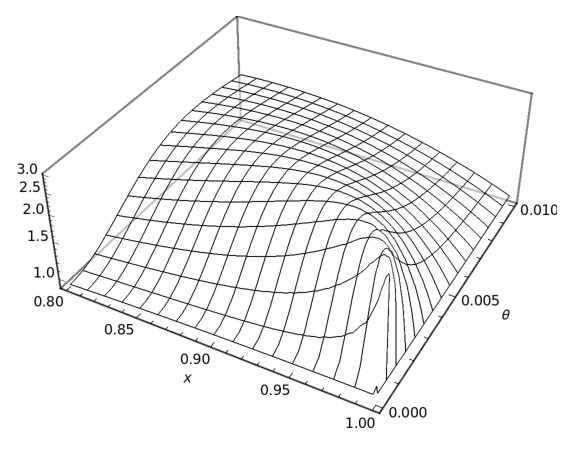
\includegraphics[scale=1]{rel-err-mj1.eps}
    %\input assets/plots/rel-err-mj1
    \caption{ Характерный вид относительной ошибки при
    аппроксимации~$f_{var}(x, \theta)$ мажорантой~$\mu_1(x,\theta)$. }
    \label{fig:mj1RelError}
\end{figure}

На рис. \ref{fig:mj1RelError} показан график относительной
ошибки $(\mu_1(x,\theta) - f(x,\theta)/f(x,\theta)$.
Относительная ошибка квадратично возрастает в области больших $\theta$, в
зависимости от $m_{A'}$ и $E_0$ достигая двух порядков величины аппроксимирующей
функции. Однако, при практическом использовании \eqref{eq:majorant1}
для генерирования значений $\tilde{x}$ необходимо иметь в виду то
обстоятельство, что большинство событий эмиссии $A'$ будут
сосредоточены в кинематической области $x \rightarrow 1, \theta \rightarrow 0$,
где $\mu_1(x, \theta)$ сравнительно точно воспроизводит поверхность
\eqref{eq:bjorkenCS}.

Первообразная по $\theta$ к ней имеет достаточно простой вид, удобный для
дальнейших преобразований:
\begin{equation}
    M_1(x) = \int \mu_1(x, \theta) \dd{\theta} = x / (2 E_0 \left[m_{A'}^2 (1 - x) - x^2 (m_e^2 + E_0^2 \theta^2) \right]).
\end{equation}

Тогда обратная функция на переменную $\theta$ через параметр $x$ и некоторое
равномерно распределённое случайное число $u \in [0, 1]$ получается
аналитически. С учётом нормировки
(для масштабных преобразований важно выдерживать относительный масштаб функций
$f_{var}(x, \theta)$ и $\mu(x, \theta)$):
\begin{equation}
    \theta^2 (u, x) = \pi^2 u \frac{ (x-1) + \frac{m_{e}^2}{m_{A'}^2} x^2 }
              { (x-1) + (\frac{m_{e}^2}{m_{A'}^2} - \pi^2 \frac{E_0^2}{m_{A'}} (1-u)) x^2 }.
    \label{eq:thetaExpr}
\end{equation}

Проинтегрировать
%$\int\limits_0^{\tilde{x}} \mu(x, \theta) d x$
$M_1(x)$
второй раз достаточно просто, однако
чтобы затем выразить переменный верхний предел понадобится разрешать
трансцендентное уравнение. Это можно либо сделать численно, либо
воспользоваться значениями $\vardbtilde{x}$ разыгранными в соответствии с той
же техникой.

\begin{figure}
    \centering
    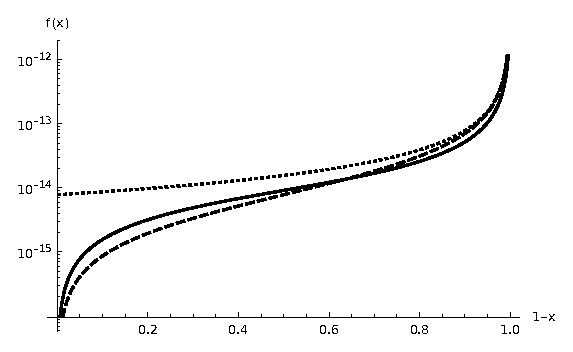
\includegraphics[scale=1]{mj1-mj2.eps}
    %\input assets/plots/rel-err-mj1
    \caption{ Характерный вид кривых, с точностью до нормирующей константы,
    соответствующих $M_1(x)$ (сплошная линия),
    $\mu_2(x)$~(короткий штрих)
    и аналитической аппроксимации интегрального по $\theta$ сечения
    $\dd{\sigma}/\dd{x}$ из \cite{bjorken}.}
    \label{fig:mj1mj2}
\end{figure}

Для этого запишем мажоранту $\mu_2(x)$ в виде:
\begin{equation}
    \mu_2(x) = ( 2 E_0^2 (m_{A'}^2 (1 - x) + m_e^2 x ) )^{-1},
\end{equation}
и получим следующие алгебраические результаты, необходимые для
разыгрывания~$x$:
\begin{align}
    M_2 = \int \mu_2(x) \dd{x} =& \frac{1}{2 E_0^2} \frac{\ln{( m_{A'}^2 (1 - x) + m_e^2 x )}}{(m_e^2 - m_{A'}^2)}, \\
    \vardbtilde{x}(u) =& \frac{1}{2 E_0^2} \frac{1-(m_e/m_{A'})^{2 u}}{1-(m_e/m_{A'})^{2}}.
    \label{eq:mj2x}
\end{align}

$M_2(x)$ упрощает поведение функции плотности вероятности
для $x$ в районе небольших переданных импульсов (см.
рис~\ref{fig:mj1mj2}), что, с учётом
относительной вероятности процесса не является важным для задач моделирования
эмиссии $A'$.

Таким образом, алгоритм получения набора случайных
чисел $\{x,\theta\}$ отвечающих плотности распределения
заданной дифференциальным сечением \eqref{eq:bjorkenCS}, сводится к следующей
последовательности операций:
\begin{enumerate}
    \item Разыграть пару равномерно распределённых в интервале $[0,1]$
        случайных чисел $\{u_1, u_2\}$. Подстановкой $u_1$ в \eqref{eq:mj2x}
        получить $\vardbtilde{x}$. Повторять до тех пор,
        пока для какой-то пары не окажется,
        что $u_2 \cdot \mu_2(\vardbtilde{x}) \le M_1 (\vardbtilde{x})$, ---
        отвечающий этому условию $\vardbtilde{x}$ следует принять за
        $\tilde{x}$.
    \item Разыграть пару равномерно распределённых в интервале $[0,1]$
        случайных чисел $\{u_3, u_4\}$. Подстановкой $u_3$ и $\tilde{x}$
        в \eqref{eq:thetaExpr} получить $\tilde{\theta}$. Если оказывается,
        что $u_4 M_1(\tilde{x}, \tilde{\theta}) > f_{var}(\tilde{x}, \tilde{\theta})$,
        необходимо повторить процедуру с п.1.
\end{enumerate}

Прошедшие процедуру псевдослучайные $\tilde{x}$ и $\tilde{\theta}$
соответствуют относительной энергии и полярному углу эмиссии $A'$ в приближении
Вайцзеккера-Вильямса, и могут использоваться при симуляциях методами
Монте-Карло. Описанный метод обладает тем важным преимуществом, что все
основные соотношения естественно параметризуются $E_0$ и не требуют дорогих
вычислений для разыгрывания во всём непрерывном спектре электромагнитного
ливня.


\begin{comment}
Выражение спектра \eqref{eq:WWSpectrum} получило широкое распространение для
описания однофотонных процессов. Однако это
приближение демонстрирует существенное расхождение в эффектах связанных со
значительным влиянием форм-факторов учитывающих распределение зарядовой
плотности в рассеивающих центрах. В работе
\cite{KimTsaiWWReview} Ким и Цай (Tsai) предлагают использовать
модифицированный метод Вайцзеккера-Вильямса для оценки дифференциальных сечений
в реакциях фотообразования аксионов на ядре, с учётом форм-факторов
ответственных за упругое и неупругое взаимодействие.
%Метод был верифицирован
%на основании точных значений дифференциальных сечений измеренных в \cite{}. slac-pub-1105 -- not found
Для целей настоящей работы
интерес представляет затем статья \cite{tsai.axion} в которой Цай
применяет авторский метод для получения количественных оценок выхода аксионов в
реакциях рассеяния тяжёлых ионов (измерения на спектрометре
EPOS~\cite{cowan.positron.1985}), --- соответствующий механизм назван
<<аксионным тормозным излучением>> (англ. \emph{axion bremsstrahlung})
и описывается диаграмой \ref{TODO}, где
%$P_1$, $P_2$, $P_i$, $P_f$ и $k$, ---
$k$ и $k'$, $p$ и $p'$ и $q$, ---
4-импульсы налетающего и рассеянного электронов, рассеивающего центра в
начальном и конечном состоянии (рассматривается в т.ч. и неупругое
взаимодействие) и аксиона, соответственно.

Оригинальную формулу работы \cite{KimTsaiWWReview}
\begin{equation}
    \left( \frac{d \sigma}{d \Omega d p} \right)_{WW} = \frac{\alpha^3}{2 \pi} \cdot
    \frac{E}{k - E} k t_{min}' ( - g_{\mu \nu} L^{\mu \nu} )_{t = t_{min}} \chi,
\end{equation}
в которой множитель $\chi$ получил название эффективного потока эквивалентных
фотонов:
\begin{equation}
    \chi = \frac{1}{2 M_i} \int\limits_{t_{min}}^{t_{max}} \frac{dt}{t^2} \int\limits_{M_i^2}^{(u-m)^2}
    d M_f^2 [(t - t_{min}) W_2 + 2 t_{min}' W_1],
\end{equation}
$M_f$ --- , $ M_i $ ---, $ L_{\mu \nu} $ ---, $g_{\mu \nu}$
% TODO: без спинов -- см ф-лу 3.17

Поскольку эти фотоны пространственноподобны, их виртуальность $t$ мала по
сравнению с прочими инвариантами задачи ($m_{A'}$), и взаимодействие электрона
с мишенью в основном определяется поперечной поляризацией. Таким образом,
кинематическое рассмотрение можно свести к задаче рассеяния на реальных фотонах
(комптоновское рассеяние, см. \cite{KimTsaiWWReview}):

\begin{equation}
\frac{d \sigma ( e(k) + Z(p) \rightarrow e(k') + A'(q) + Z(p') )}{ dE_{A'} d \cos \theta_{A'} } =
    \frac{ \alpha \chi }{ \pi } \frac{E_0 x \beta_{A'}}{1 - x} \frac{ d \sigma (p + q \rightarrow p' + k) }{d (p k)},
\end{equation}

где $x = E_{A'}/E_0$, $t = - q^2$, $\beta_{A'} = \sqrt(1 - m_{A'}^2/E_0^2)$.

%В числе прочего обсуждается, что механизм Примакова пренебрежимо мал по вкладу
%по сравнению с тормозным.

% TODO: ...
\end{comment}

\subsection{Оценки выхода сигнального события}

Согласно выражению дифференциального сечения~\eqref{eq:bjorkenCS}
в работе~\cite{bjorken} приблизительное количество
образовавшихся~$A'$:
\begin{equation}
    N_{A'} \approx N_e C' \epsilon^2 \frac{m^2}{m^2_{A'}}, \quad C' \simeq 10.
    \label{eq:aprime-yield-approx}
\end{equation}

В постановке эксперимента важно учесть характерное время
жизни гипотетической частицы, поскольку распадной длины может
быть недостаточно для покидания активной мишени. Характерная
(средняя) длина распада согласно~\cite{bjorken}:
\begin{equation}
    l_0 \approx 0{,}8 \text{см} \cdot \frac{E_0 / 10 ~\text{ГэВ}}{N_{eff}}
        \left( \frac{10^{-4}}{\epsilon} \right)^2 \left( \frac{100~\text{МэВ}}{m_{A'}} \right)^2.
    \label{eq:aprime-decay-length}
\end{equation}

Выражения \eqref{eq:aprime-yield-approx} и \eqref{eq:aprime-decay-length}
позволяют грубо оценить примерный выход реакции в свинцовой мишени,
учитывая геометрические ограничения на длину мишени. Результаты
такой оценки выполненной для $\epsilon = 10^{-4}$ и $N_{e} = 10^{14}$ приведены в
таблице~\ref{tab:aprime-geom-yield-estimations}, где
$m_{A'}$ -- гипотетическая масса тёмного фотона,
$N_{prod}$ -- число родившихся $A'$ в толстой мишени ($C'\approx 10$),
$l_{1/2} = l_0 \text{ln}~2 \approx 0{,}693 ~ l_0$ -- длина
на которой распадается половина~$A'$,
$P_{dec}$ -- примерная доля распавшихся частиц при длине распадной базы
в $1~\mathrm{м}$,
$N_{obs}$ -- число наблюдаемых распадов ниже по пучку.

\begin{table}[h]
\centering
\begin{tabular}{r|ccccc}
 $m_{A'}$, ГэВ & $N_{prod}$ & $l_{1/2}$, см & $P_{dec}$ & $N_{obs}$ \\ \hline
$0{,}01$ & $261$        & $555$    &  $0{,}118$ & $30{,}7$ \\
 $0{,}1$ & $2{,}61$     & $5{,}5$  &  $1$       & $2{,}61$ \\
 $0{,}5$ & $0{,}104$    & $0{,}2$  &  $1$       & $0{,}104$ \\
     $1$ & $0{,}0261$   & $0{,}05$ &  $1$       & $0{,}0261$
\end{tabular}
\caption{Оценка согласно \eqref{eq:aprime-yield-approx} и \eqref{eq:aprime-decay-length}}
\label{tab:aprime-geom-yield-estimations}
\end{table}
%\begin{flushleft}
%\footnotesize\textit{Примечания.} (i) $N_{\rm prod}\approx N_e\,C'\,\varepsilon^2(m_e^2/m_{A'}^2)$, $C'\simeq 10$ (толстая мишень). (ii) $\ell_0\simeq 0.8~\mathrm{см}\cdot\frac{E_0/10~\mathrm{GeV}}{N_{\!eff}}\left(\frac{10^{-4}}{\varepsilon}\right)^2\!\left(\frac{100~\mathrm{MeV}}{m_{A'}}\right)^2$. (iii) Если распадной объём начинается \emph{после} экрана длиной $S$, используйте $P=e^{-S/\ell_0}\bigl(1-e^{-L/\ell_0}\bigr)$. (iv) При $m_{A'}\ge 2m_\mu$ разумно брать $N_{\!eff}\gtrsim 2$, что уменьшит $\ell_0$ и увеличит $P$.
%\end{flushleft}

Из таблицы~\ref{tab:aprime-geom-yield-estimations} видно, что установка
с толщиной активной мишени в несколько десятков сантиметров и распадной
базой порядка метра и более в состоянии зарегистрировать десятки
частиц с массами до сотни МэВ и константой связи более $10^{-4}$.

Более точные оценки чувствительности эксперимента для этой и других
теоретических моделей, включающие более точный учёт форм-фактора,
подробно изложены в работе~\cite{voronchihin2025}.
